% !TEX program = xelatex
\documentclass[11pt, a4paper]{article}
\usepackage{tikz}
\usetikzlibrary{decorations.pathmorphing}

\begin{document}

\section{Decoration Shapes}

Try changing the decoration name to: \texttt{snake}, \texttt{zigzag},
\texttt{coil}, or \texttt{bumps}.

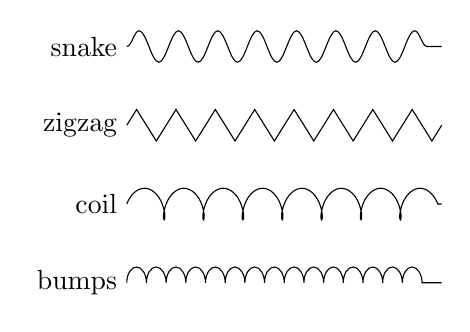
\begin{tikzpicture}
  % Snake
  \draw[decorate, decoration={snake, amplitude=2mm, segment length=5mm}]
    (0,0) -- (4,0);
  \node[left] at (0,0) {snake};

  % Zigzag
  \draw[decorate, decoration={zigzag, amplitude=2mm, segment length=5mm}]
    (0,-1) -- (4,-1);
  \node[left] at (0,-1) {zigzag};

  % Coil
  \draw[decorate, decoration={coil, amplitude=2mm, segment length=5mm}]
    (0,-2) -- (4,-2);
  \node[left] at (0,-2) {coil};

  % Bumps
  \draw[decorate, decoration={bumps, amplitude=2mm, segment length=5mm}]
    (0,-3) -- (4,-3);
  \node[left] at (0,-3) {bumps};
\end{tikzpicture}

\end{document}
